% -----------------------------------------------------------------------------
% ########################
% # PREDLOGA ZA POROCILO #
% ########################
%
% @author Iztok Starc
% @date   3. december 2008
%
\documentclass[a4paper,12pt]{report}

% -----------------------------------------------------------------------------
% ####################################################
% # UPORABA PAKETOV - NASTAVITEV JEZIKA in KODIRANJA #
% ####################################################
\usepackage[slovene]{babel}
\usepackage[utf8]{inputenc}
\usepackage{lmodern}
\usepackage[T1]{fontenc}
\usepackage[sc]{mathpazo}
\linespread{1.05}
\usepackage[T1]{fontenc}

% -----------------------------------------------------------------------------
% ######################################
% # VNOS KLJUCNIH PARAMETROV BESEDILA  #
% ######################################

\newcommand{\naslov}     {Spletna trgovina}
\newcommand{\prviavtor}  {Jaka Stavanja}
\newcommand{\prviindeks} {63150270}
\newcommand{\drugiavtor} {Blaž Rupnik}
\newcommand{\drugiindeks}{63150253}
\newcommand{\kraj}       {Ljubljana}

% -----------------------------------------------------------------------------
% ###################
% # UPORABA PAKETOV #
% ###################
\usepackage[a4paper,left=25mm,right=25mm,top=20mm,bottom=30mm,includehead]{geometry}

\usepackage{graphicx, epsfig}

\usepackage{fancyhdr}

\usepackage[
colorlinks=true, linkcolor=blue, citecolor=red,
%
pdftitle={\naslov},
pdfauthor={\prviavtor, \drugiavtor},
pdfsubject={Poročilo seminarske naloge pri predmetu Elektronsko Poslovanje},
pdfkeywords={spletna prodajalna, PHP, SSL, MySQL}, a4paper, pagebackref=true, unicode]{hyperref}

% -----------------------------------------------------------------------------
\begin{document}

% -----------------------------------------------------------------------------
% ##################
% # NASLOVNA STRAN #
% ##################
\begin{titlepage}
	\begin{center}
	{UNIVERZA V LJUBLJANI\\[10pt] 
	FAKULTETA ZA RAČUNALNIŠTVO IN INFORMATIKO}

	\vspace{65mm}

	{\Large\textbf{\naslov}}

	\vspace{10mm}

	{\large Poročilo seminarske naloge pri predmetu\\[10pt] Elektronsko poslovanje}

	\vfill
	\vspace{60mm}

\hspace{20mm}
\begin{minipage}[t]{70mm}
	{\bf Študenti}\\
	{\prviavtor} ({\prviindeks})\\ 
	{\drugiavtor} ({\drugiindeks})
\end{minipage}
%\hfill
\begin{minipage}[t]{50mm}
	{\bf Mentor}\\
	David Jelenc
\end{minipage}
%\hspace{20mm}

	\vspace{35mm}

	{	\kraj, \today}
	\end{center}
\end{titlepage}

% -----------------------------------------------------------------------------
% ##################
% # KAZALO VSEBINE #
% ##################

\tableofcontents

% -----------------------------------------------------------------------------
% ############
% # POVZETEK #
% ############
%\begin{abstract}
%\end{abstract}

% -----------------------------------------------------------------------------
% ##################
% # UVOD DOKUMENTA #
% ##################
\chapter{Uvod}

Pri predmetu Elektronsko poslovanje smo imeli nalogo narediti varno enostavno spletno trgovino s poudarkom na temah, ki smo jih spoznavali skozi semester na vajah tega predmeta. Odločila sva se narediti preprosto trgovino z oblačili. Za izdelavo sva uporabila naslednje tehnologije: PHP, MySQL, Apache, CSS (knjižnica Bulma), Javascript (knjižnice Axios, Flickity) ter Javo in Android Studio za Android odjemalca. Za učinkovito in vzporedno delo sva uporabljala tehnologijo Git.

Podatkovni model sva izdelala z MySQL Workbench-om. 

% -----------------------------------------------------------------------------
% ###################
% # JEDRO DOKUMENTA #
% ###################

% -----------------------------------------------
\chapter{Navedba realiziranih storitev}

Implementirala sva naslednje razširjene storitve:

\begin{itemize}
    \item Registracija strank z uporabo filtriranja CAPTCHA.
    \item Smiselna organizacija in izvedba uporabniškega vmesnika s pomočjo tehnologij kot so CSS in JavaScript ter uporaba AJAX.
\end{itemize}


% -----------------------------------------------
\chapter{Podatkovni model}

Slika logičnega podatkovnega modela (generirana z MySQL Workbench programom).
\newline
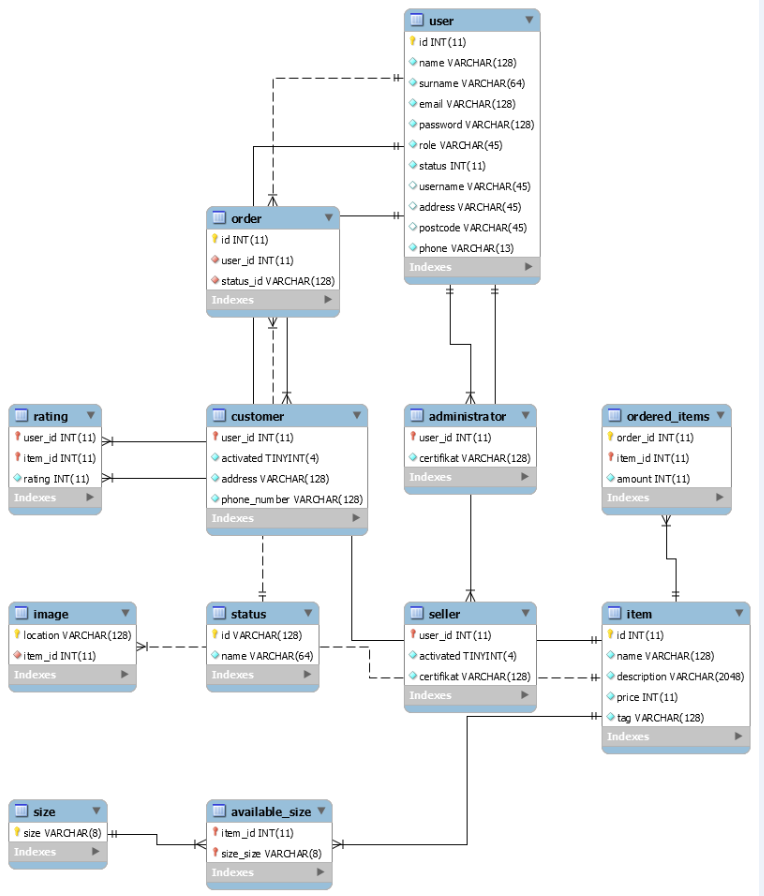
\includegraphics[scale=0.9]{images/database_model_diagram.png}
\newpage
Najin podatkovni model je sestavljen iz sledečih tabel:
\begin{itemize}
    \item User
    \item Administrator
    \item Seller
    \item Customer
    \item Order
    \item Rating (Na koncu te tabele nisva uporabila)
    \item Image (Na koncu te tabele nisva uporabila)
    \item Size (Na koncu te tabele nisva uporabila)
    \item Available size (Na koncu te tabele nisva uporabila)
    \item Item
    \item Ordered items
    \item Status
\end{itemize}
% -----------------------------------------------
\chapter{Varnost sistema}

Opišite implementirane mehanizme za nadzor dostopa ter ostale kontrole, ki ste jih implementirali. Pri vsake navedite, kaj je njen namen oz. katere varnostne grožnje preprečuje.

% -----------------------------------------------
\chapter{Izjava o avtorstvu seminarske naloge}

Spodaj podpisani \textit{\prviavtor}, vpisna številka \textit{\prviindeks}, sem (so)avtor seminarske naloge z naslovom \textit{\naslov}. S svojim podpisom zagotavljam, da sem izdelal ali bil soudeležen pri izdelavi naslednjih sklopov seminarske naloge:
\begin{itemize}
    \item Spletna aplikacija
\end{itemize}

Podpis: {\prviavtor}, l.r.

\newpage

Spodaj podpisana \textit{\drugiavtor}, vpisna številka \textit{\drugiindeks}, sem (so)avtor seminarske naloge z naslovom \textit{\naslov}. S svojim podpisom zagotavljam, da sem izdelal ali bil soudeležen pri izdelavi naslednjih sklopov seminarske naloge:
\begin{itemize}
    \item Izdelava Android odjemalca
    \item Pomoč pri spletni aplikaciji
\end{itemize}

Podpis: {\drugiavtor}, l.r.

% -----------------------------------------------------------------------------
% #######################
% # ZAKLJUCEK DOKUMENTA #
% #######################
\chapter{Zaključek}

Izdelava spletne trgovine se je izkazalo za izzivalno vendar zanimivo delo. Podrobneje sva se spoznala z uporabljenimi tehnologijami ter njihovim delovanjem. Želela sva narediti več razširjenih storitev vendar nama je zmanjkalo časa (zato so tudi nekate tabele na koncu ostale neuporabljene). Kot eno najboljših nadgradenj predvsem vidiva serviranje slik za vsak izdelek, tako na spletni aplikaciji kot na Android odjemalcu, saj pri trenutni trgovini to predstavlja kot eno glavnih pomanjkljivosti.


\end{document}
